% !TeX root = ../../../book.tex

\subsection{函数复合}

\subsubsection*{引言}

考虑函数的示意图:设函数 $f : A \to B$ 和 $g : B \to C$,它们的定义如下:

\begin{multicols}{2}
    \begin{center}
        {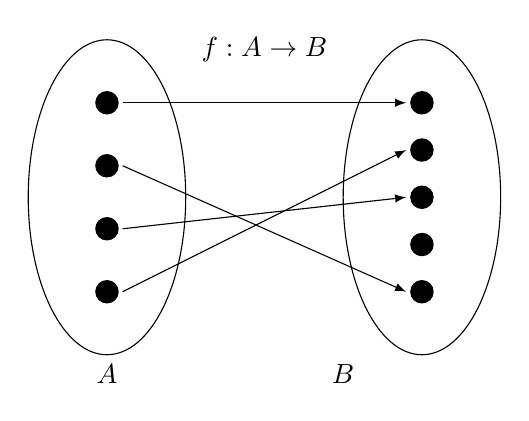
\begin{tikzpicture}[scale=1]
                \foreach \x in {0,...,4}
                    {
                        \node at (4, -\x*0.6)[circle,fill,inner sep=3pt]{};
                    }
                \draw (4,-1.2) ellipse (1 and 2);

                \foreach \x in {0,...,3}
                    {
                        \node at (0, -\x*0.8)[circle,fill,inner sep=3pt]{};
                    }
                \draw (0,-1.2) ellipse (1 and 2);

                \draw[-latex] (0.2,-0.0) -- (3.8,0.0);
                \draw[-latex] (0.2,-0.8) -- (3.8,-2.4);
                \draw[-latex] (0.2,-1.6) -- (3.8,-1.2);
                \draw[-latex] (0.2,-2.4) -- (3.8,-0.6);

                \node[below] at (0, -3.2){$A$};
                \node[below] at (3, -3.2){$B$};
                \node[above] at (2, 0.4){$f:A \to B$};
            \end{tikzpicture}}
    \end{center}

    \begin{center}
        {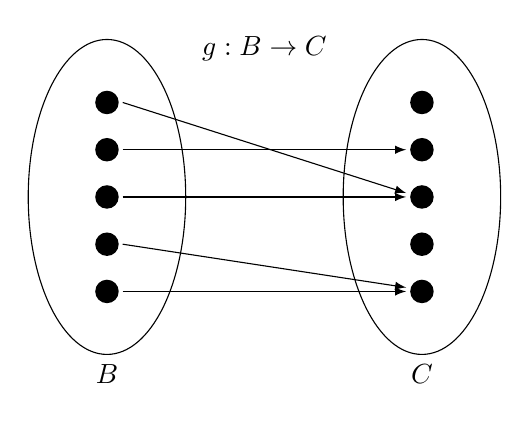
\begin{tikzpicture}[scale=1]
                \foreach \x in  {0,...,4}
                    {
                        \node at (4, -\x*0.6)[circle,fill,inner sep=3pt]{};
                    }
                \draw (4,-1.2) ellipse (1 and 2);

                \foreach \x in  {0,...,4}
                    {
                        \node at (0, -\x*0.6)[circle,fill,inner sep=3pt]{};
                    }
                \draw (0,-1.2) ellipse (1 and 2);

                \draw[-latex] (0.2,-0.0) -- (3.8,-1.15);
                \draw[-latex] (0.2,-0.6) -- (3.8,-0.6);
                \draw[-latex] (0.2,-1.2) -- (3.8,-1.2);
                \draw[-latex] (0.2,-1.8) -- (3.8,-2.35);
                \draw[-latex] (0.2,-2.4) -- (3.8,-2.4);

                \node[below] at (0, -3.2){$B$};
                \node[below] at (4, -3.2){$C$};
                \node[above] at (2, 0.4){$g:B \to C$};
            \end{tikzpicture}}
    \end{center}
\end{multicols}

直观感觉,$f$ 就像一张``地图'',为我们提供了从 $A$ 中元素到 $B$ 中元素的特定路线,而 $g$ 则是从 $B$ 中元素到 $C$ 中元素的``地图''。如果我们依次遵循这些``地图'',会发生什么呢?也就是说,让我们把这两张``地图''叠加起来,

\begin{center}
    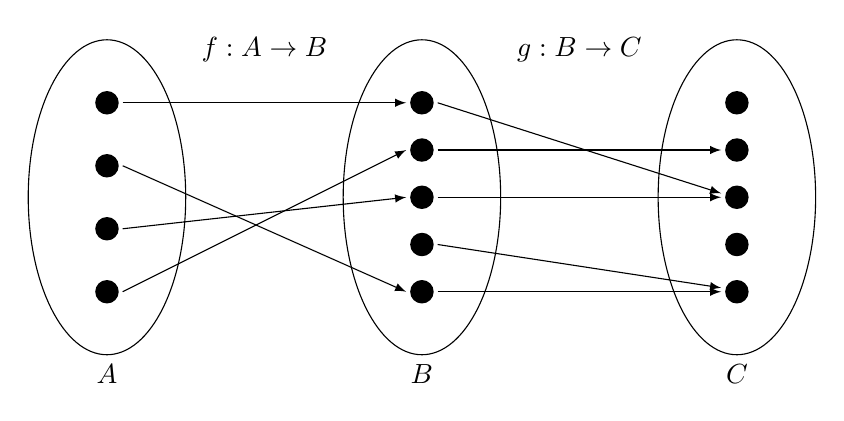
\begin{tikzpicture}[scale=1]
        \foreach \x in {0,...,3}
            {
                \node at (0, -\x*0.8)[circle,fill,inner sep=3pt]{};
            }
        \draw (0,-1.2) ellipse (1 and 2);

        \foreach \x in {0,...,4}
            {
                \node at (4, -\x*0.6)[circle,fill,inner sep=3pt]{};
            }
        \draw (4,-1.2) ellipse (1 and 2);

        \foreach \x in  {0,...,4}
            {
                \node at (8, -\x*0.6)[circle,fill,inner sep=3pt]{};
            }
        \draw (8,-1.2) ellipse (1 and 2);

        \draw[-latex] (0.2,-0.0) -- (3.8,0.0);
        \draw[-latex] (0.2,-0.8) -- (3.8,-2.4);
        \draw[-latex] (0.2,-1.6) -- (3.8,-1.2);
        \draw[-latex] (0.2,-2.4) -- (3.8,-0.6);

        \draw[-latex] (4.2,-0.0) -- (7.8,-1.15);
        \draw[-latex] (4.2,-0.6) -- (7.8,-0.6);
        \draw[-latex] (4.2,-1.2) -- (7.8,-1.2);
        \draw[-latex] (4.2,-1.8) -- (7.8,-2.35);
        \draw[-latex] (4.2,-2.4) -- (7.8,-2.4);

        \node[below] at (0, -3.2){$A$};
        \node[below] at (4, -3.2){$B$};
        \node[below] at (8, -3.2){$C$};
        \node[above] at (2, 0.4){$f:A \to B$};
        \node[above] at (6, 0.4){$g:B \to C$};
    \end{tikzpicture}
\end{center}

然后省略中间环节,可直接得到从 $A$ 到 $C$ 的映射:

\begin{center}
    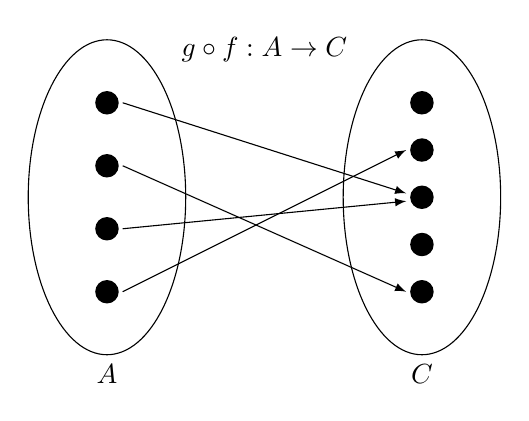
\begin{tikzpicture}[scale=1]
        \foreach \x in {0,...,4}
            {
                \node at (4, -\x*0.6)[circle,fill,inner sep=3pt]{};
            }
        \draw (4,-1.2) ellipse (1 and 2);

        \foreach \x in {0,...,3}
            {
                \node at (0, -\x*0.8)[circle,fill,inner sep=3pt]{};
            }
        \draw (0,-1.2) ellipse (1 and 2);

        \draw[-latex] (0.2,-0.0) -- (3.8,-1.15);
        \draw[-latex] (0.2,-0.8) -- (3.8,-2.4);
        \draw[-latex] (0.2,-1.6) -- (3.8,-1.25);
        \draw[-latex] (0.2,-2.4) -- (3.8,-0.6);

        \node[below] at (0, -3.2){$A$};
        \node[below] at (4, -3.2){$C$};
        \node[above] at (2, 0.4){$g \circ f:A \to C$};
    \end{tikzpicture}
\end{center}

这是否合理?当然是合理的!对于数学对象,我们总是关注其组合、操作与推广的可能性。函数的这种组合称为\textbf{复合}。需注意,仅当第一个函数的值域与第二个函数的定义域一致时,复合才有意义,这一点将在定义中体现。

\subsubsection*{定义}

\begin{definition}
    设 $A, B, C$ 为集合,$f : A \to B$ 和 $g : B \to C$ 为函数。定义函数 $h : A \to C$ 为:
    \[\forall a \in A \centerdot h(a) = g(f(a))\]
    
    我们称 $h$ 是 $g$ 和 $f$ 的\dotuline{复合},记作 $g \circ f$。

    亦可将该术语简称为 $f$ 是 ``$g$ 复合 $f$''。
\end{definition}

该定义整合了我们之前提到的所有概念。要求函数 $f$(``第一个''函数)的值域必须是函数 $g$(``第二个''函数)的定义域。

函数可以直观地理解为\emph{机器}或\emph{黑箱}:输入定义域元素,输出值域元素,内部过程未知。若将实现 $f$ 的机器与实现 $g$ 的机器相连,使 $f$ 的输出成为 $g$ 的输入,则最终输出是集合 $C$ 的元素。此联合系统即为\emph{复合} $g \circ f$ 的直观体现——它构成了一台按序执行操作的新机器。

\subsubsection*{符号}

注意符号 $g \circ f$ 的顺序与实际函数应用顺序的对应关系:先应用 $f$,再应用 $g$,即 $g(f(a))$。用语言描述时,可将``$g(f(a))$''读作``$a$ 先经过 $f$ 再经过 $g$''。事实上,如果你发现自己难以记住这个顺序,建议将``$\circ$''读作``在……之后'',因此 $h = g \circ f$ 表示``$g$ 在 $f$ 之后'',因为先对元素 $a$ 应用 $f$,再应用 $g$。

记住复合函数的符号至关重要,并且要区分函数 $g \circ f$ 本身和将其应用于元素 $x \in A$ 的区别。例如,用``$\circ$''符号表示``$x$ 先应用 $f$ 再应用 $g$''时,应写做:
\[(g \circ f)(x)\]
这是将函数 $g \circ f$ 应用于元素 $x$。然而,以下写法\textbf{无意义},因为它混淆了函数与元素的概念:
\[g \circ f(x)\]
你能看出区别吗?$f(x)$ 是 $f$ 值域 $B$ 中的一个元素,而 $g$ 是函数。将函数直接与元素复合没有意义。当复合多个函数时(例如 $(h \circ (g \circ k) \circ f)(z)$,其中 $z$ 是 $f$ 定义域的元素,而 $f,g,h,k$ 均为函数),这种区分尤为重要。

\subsubsection*{示例}

\begin{example}
    定义函数 $ C : \mathbb{R} \to \mathbb{R}$ 为
    \[\forall x \in \mathbb{R} \centerdot C(x) = x - 273.15\]

    定义函数 $ F : \mathbb{R} \to \mathbb{R}$ 为
    \[\forall x \in \mathbb{R} \centerdot F(x) = \frac{9}{5}x + 32\]

    函数 $C$ 将开尔文温度转换为摄氏温度。

    函数 $F$ 将摄氏温度转换为华氏温度。

    函数 $F \circ C$ 直接将开尔文温度转换为华氏温度。我们可以通过复合函数``规则''从而得到直接转换公式。
    \begin{align*}
        \forall x \in \mathbb{R} \centerdot (F \circ C)(x) & = F(C(x)) = F(x - 273.15)                                  \\
                                                           & = \frac{9}{5} \cdot (x - 273.15) + 32 = \frac{9}{5}-459.67
    \end{align*}
\end{example}

\begin{example}
    设函数 $f : \mathbb{R} \to \mathbb{Z}$ 定义为
    \[\forall x \in \mathbb{R} \centerdot f(x) = \lfloor x \rfloor\]

    ($\lfloor x \rfloor$ 表示 $x$ 向下取整:即满足 $z \le x$ 的\emph{最大}整数 $z \in \mathbb{Z}$。)

    设函数 $g : \mathbb{Z} \to \mathbb{N}$ 定义为
    \[\forall z \in \mathbb{Z} \centerdot g(z) = \begin{cases}
            -z  & \text{如果}\;z<0     \\
            z+1 & \text{如果}\;z \ge 0
        \end{cases}\]

    求 $g \circ f$。

    注意,若 $x \in \mathbb{R} < 0$,则 $\lfloor x \rfloor < 0$。若 $x \in \mathbb{R} \ge 0$,则 $\lfloor x \rfloor \ge 0$。这表明 $g \circ f$ 是一个\textbf{分段}函数:
    \[\forall x \in \mathbb{R} \centerdot (g \circ f)(x) = \begin{cases}
            -\lfloor x \rfloor  & \text{若\ } z<0     \\
            \lfloor x \rfloor+1 & \text{若\ } z \ge 0
        \end{cases}\]

    问题:这个函数是单射吗?是满射吗?请尝试证明你的结论。
\end{example}

\begin{example}
    定义函数 $f : \mathbb{N} \to \mathbb{N}, g : \mathbb{Z} \to \mathbb{N}, h : \mathbb{Z} \to \mathbb{N}$ 为:
    \begin{align*}
        \forall n \in \mathbb{N} \centerdot f(n) & = n + 3  \\
        \forall n \in \mathbb{N} \centerdot g(n) & = n^2    \\
        \forall n \in \mathbb{N} \centerdot h(n) & = 2n - 1
    \end{align*}
    
    (问题:你确定这些函数都是良好定义的吗?为什么?)

    我们可以得到 $g \circ f$ 和 $h \circ g$ 的``规则'':
    \begin{align*}
        \forall n \in \mathbb{N} \centerdot (g \circ f)(n) & = g(f(n)) = g(n + 3) = (n + 3)^2 = n^2 + 6n + 9 \\
        \forall n \in \mathbb{N} \centerdot (h \circ g)(n) & = h(g(n)) = h(n^2) = 2n^2-1
    \end{align*}

    甚至由此可得进一步复合的规则,比如 $h \circ (g \circ f)$:
    \begin{align*}
        \forall n \in \mathbb{N} \centerdot \left(h \circ (g \circ f)\right)(n) & = h\left((g \circ f)(n)\right) = h(n^2 + 6n + 9) \\
                                                                             & = 2(n^2 + 6n + 9) - 1                         \\
                                                                             & = 2n^2 + 12n + 17
    \end{align*}

    类似地,也可以得到 $(h \circ g) \circ f$ 的规则:
    \begin{align*}
        \forall n \in \mathbb{N} \centerdot \left((h \circ g) \circ f\right)(n) & = (h \circ g)(f(n)) = (h \circ g)(n + 3) \\
                                                                             & = 2(n + 3)^2 - 1 = 2(n^2 + 6n + 9) - 1   \\
                                                                             & = 2n^2 + 12n + 17
    \end{align*}
\end{example}

考察上面两个结果,发现二者\textbf{相等}!也就是说,从\emph{函数}意义上讲,我们刚刚通过证明在\emph{每个}允许的输入上都能产生相同的输出,从而\emph{证明}了
\[h \circ (g \circ f) = (h \circ g) \circ f\]

\subsubsection*{复合结合律}

在前面的例子中,函数 $f, g, h$ 并无特殊之处。实际上,所得结果在\emph{一般情形下}均成立。以下定理和证明将阐明这一点——函数复合满足\textbf{结合律},即进行多重函数复合时,括号的位置不影响最终结果。

\begin{theorem}
    设 $A,B,C D$ 为任意集合。设 $f : A \to B, g : B \to C, h : C \to D$ 为函数。则
    \[h \circ (g \circ f) = (h \circ g) \circ f\]
\end{theorem}

\begin{proof}
    我们要证明对于任意可能的输入,函数 $(h \circ g) \circ f$ 和函数 $h \circ (g \circ f)$ 的输出相同。

    给定 $x \in A$,应用\emph{复合}的定义,可得
    \[[h \circ (g \circ f)](x) = h\left((g \circ f)(x)\right) = h\left(g(f(x))\right)\]
    \[[(h \circ g) \circ f](x) = \left(h \circ g\right)(f(x)) = h\left(g(f(x))\right)\]
\end{proof}

\subsubsection*{复合与映射}

现在考虑一个有趣的问题:若将两个具有相同性质的函数复合,该性质是否依然存在?例如,复合两个单射函数后,结果是否仍为单射?是否只需其中一个函数为单射,复合函数即为单射?

同理,对于两个函数的复合,若已知复合函数是满射,能否断定其中一个函数必为满射?还是说两个函数都必须是满射?

本小节将陈述并证明这些问题的若干结论,并在本节及本章末尾的练习中要求你证明相关事实或构造反例。

\begin{proposition}
    设 $A, B, C$ 为集合,$f : A \to B$ 和 $g : B \to C$ 为函数。若 $g \circ f$ 为单射,则 $f$ 必为单射。
\end{proposition}

(请注意,此处并未假设 $g$ 具有任何特定性质;$g$ 甚至未必是单射!作为练习,请尝试构造两个函数 $f: A \to B$ 和 $g: B \to C$ 的实例:一例中 $g \circ f$ 与 $g$ 均为单射;另一例中 $g \circ f$ 是单射但 $g$ 不是单射。)

\begin{proof}
    对任意给定 $x,y \in A$,假设 $f(x)=f(y)$,我们要证明 $x=y$。

    因为 $g$ 是良好定义的函数,所以 $g(f(x)) = g(f(y))$。

    这意味着 $(g \circ f)(x) = (g \circ f)(y)$。

    因为 $g \circ f$ 为单射,所以 $x=y$。证毕。
\end{proof}

请注意,上述命题的\emph{逆命题}并不成立。因为该命题涉及一般函数,所以只需提供一个反例即可证伪。

\begin{proposition}
    设 $A, B, C$ 为集合,$f : A \to B$ 和 $g : B \to C$ 为函数。若 $f$ 为单射,则 $g \circ f$ 不一定为单射。
\end{proposition}

在阅读我们提供的反例之前,试着自己动手构造一个反例。切记,反例无需复杂,满足条件即可!

\begin{proof}
    构造反例如下:

    定义 $A = \{1, 2\}, B = \{\heartsuit, \diamondsuit\}, C = \{\bigstar\}$。

    定义函数 $f$ 为 $f(1) = \heartsuit, f(2) = \diamondsuit$。

    显然 $f$ 为单射,因为 $f(1) \ne f(2)$。

    定义函数 $g$ 为 $g(1) = g(2) = \bigstar$ 。

    则 $g \circ f$ 定义为 
    \begin{align*}
        (g \circ f)(1) &= \bigstar \\
        (g \circ f)(2) &= \bigstar
    \end{align*}

    这表明 $g \circ f$ 不是单射,因为 $(g \circ f)(1) = (g \circ f)(2)$,而 $1 \ne 2$。
\end{proof}

\clearpage